\begin{frame}
\frametitle{No Free Ducklings}
{\bf No Free Lunch theorem} says that learning is impossible without prior knowledge (\url{http://en.wikipedia.org/wiki/No\_free\_lunch\_in\_search\_and\_optimization}).

{\bf Ugly Duckling theorem} says that things are all equivalently similar to each other without prior knowledge (\url{http://en.wikipedia.org/wiki/Ugly\_duckling\_theorem}).

\vspace{1cm}
What prior knowledge do we have about the variability among people that can be measured using MRI?

How do we use this knowledge?
\end{frame}

\begin{frame}
\frametitle{Different ways of measuring distances}
\begin{columns}[c]
\column{.3\textwidth}
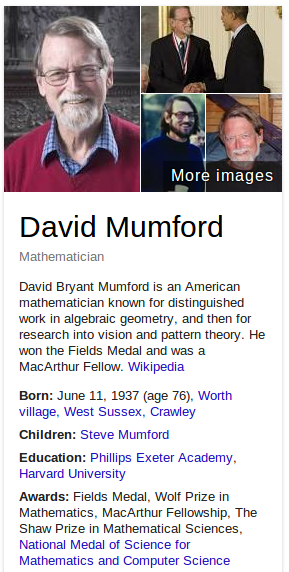
\includegraphics[width=\textwidth]{mumford}
\column{.7\textwidth}
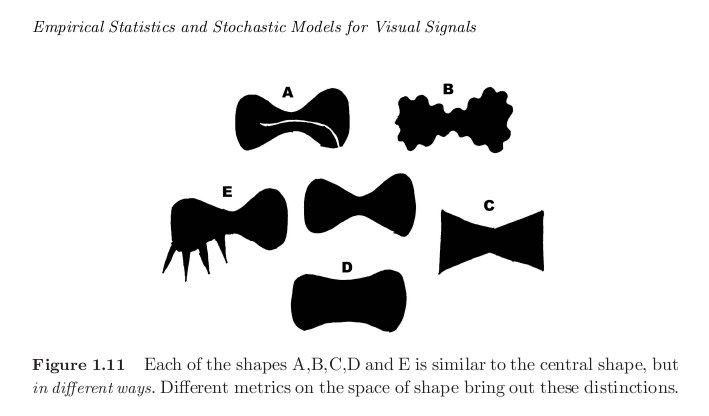
\includegraphics[width=\textwidth]{mumford_fig}
\end{columns}
\end{frame}

%\begin{frame}
%\frametitle{Different ways of measuring distances}
%\begin{columns}[c]
%\column{.2\textwidth}
%\begin{center}
%Two simulated images\par
%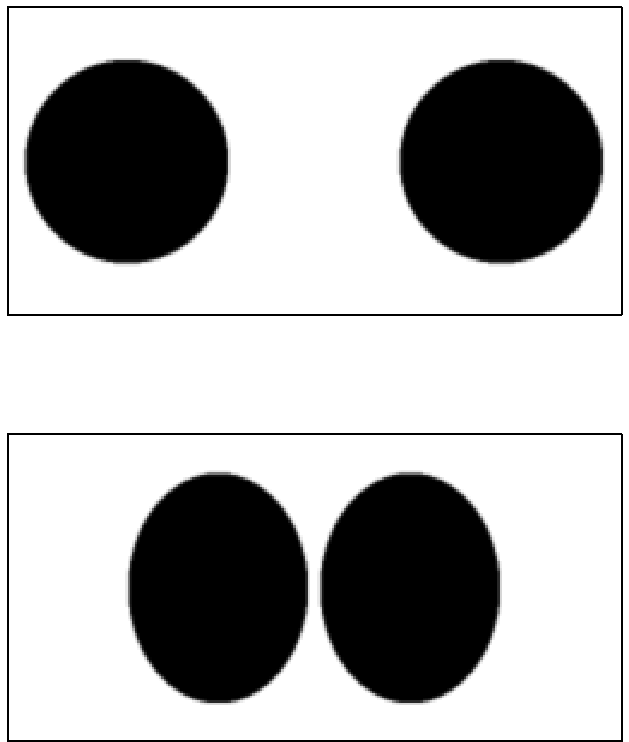
\includegraphics[width=\textwidth]{figure2Di}
%\end{center}
%\column{.8\textwidth}
%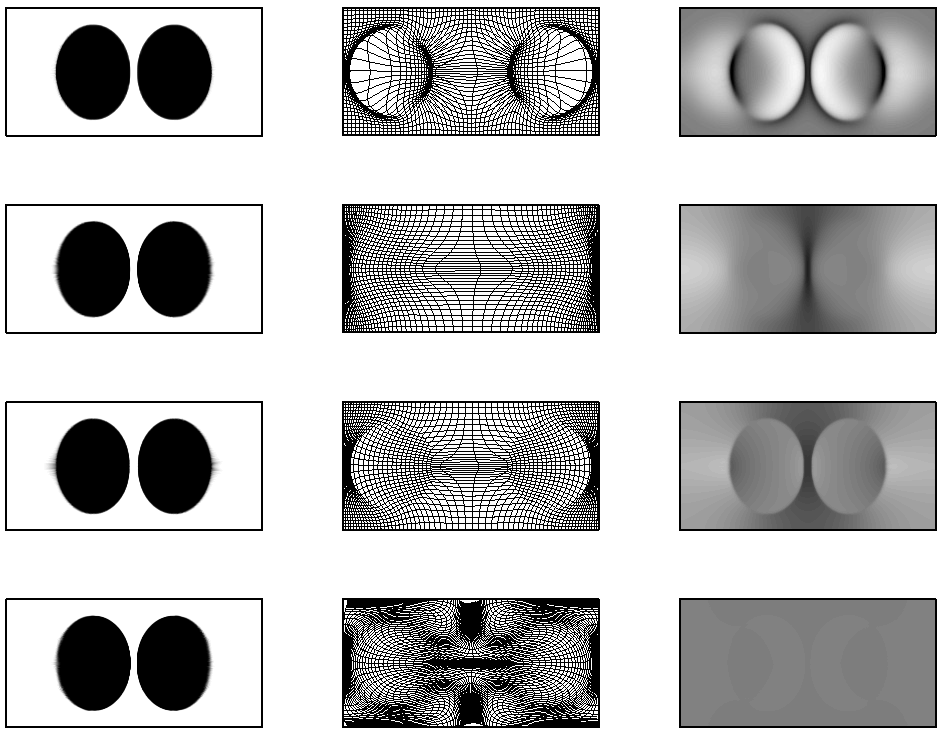
\includegraphics[width=\textwidth]{figure2Dii}
%\end{columns}
%\end{frame}

\begin{frame}
\frametitle{Weighting the data}
\begin{Huge}
\begin{align*}
{\bf K} = {\bf X}{\bf W}{\bf X}^T
\end{align*}
\end{Huge}
\end{frame}

\begin{frame}
\frametitle{Prior knowledge about brain regions involved}
\begin{itemize}
\item The best way would be to augment the training data with data from previous studies.
\item Lack of data-sharing means this is generally not possible,\\
      so we need to extract information from publications.
\item The neuroimaging literature is mostly blobs.
\item These give pointers about how best to weight the data\\
      (${\bf W} = diag({\bf w}), w_i \in \mathbb{R}^+$).
\end{itemize}
\end{frame}

\begin{frame}
\frametitle{Weighting suspected regions more heavily}
\begin{center}
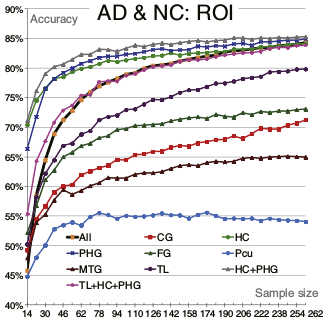
\includegraphics[width=.45\textwidth]{prior_knowledge_AD_NC}
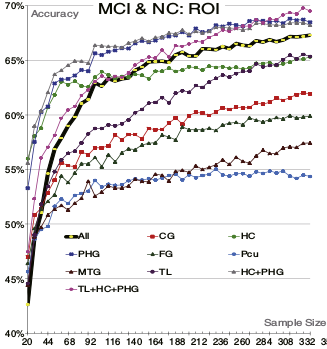
\includegraphics[width=.45\textwidth]{prior_knowledge_MCI_NC}\par
\begin{tiny}
Chu et al. ``Does feature selection improve classification accuracy? Impact of sample size and feature selection on classification using anatomical magnetic resonance images''.  NeuroImage 60:59--70 (2012).\par
\end{tiny}
\end{center}
\end{frame}

